% Chapter Template

\chapter{Background} 

\label{Chapter2} % Change X to a consecutive number; for referencing this chapter elsewhere, use \ref{ChapterX}

%\lhead{Chapter 2. \emph{Understanding the domain}} % Change X to a consecutive number; this is for the header on each page - perhaps a shortened title

%----------------------------------------------------------------------------------------
%	SECTION 1
%----------------------------------------------------------------------------------------

\section{Understanding the domain}

\subsection{Immune system and antibodies }

The immune system is the central part of the human body responsible for protection against infections. In order to function properly, the immune system has to detect a wide range of threats, and at the same time distinguish them from  healthy tissue. The main weapon the immune system can use are antibodies.   \\

The antibody is a protein complex produced by \textit{B cells} \footnote{ a subgroup of white blood cells, a viral part of the immune system} that initiates an immune response against a target antigen \footnote{Foreign substance that, when introduced into the body, is capable of stimulating an immune response}. Their primal role is to recognize the unique part of the foreign target and  protect the body from infections. The basic organization of the antibody includes two functional domains that, together, resemble the letter Y (Figure \ref{fig:AntibodyIllustration}, left). The \textit{Fab}  part makes up the arms of the Y, and it contains the antigen-binding site - the region responsible for antigen binding. The \textit{Fc} part comprises the tail of the Y and effects other cells, proteins and antibodies.  \\

This unique structure allows detection of antigens, in direct or indirect manner. By direct detection we assume detection using a single fluorophore-labeled antibody, and by indirect detection we assume detection through binding of a fluorophore-labeled secondary antibody raised against the Fc part of an unlabeled primary antibody (as illustrated in Figure \ref{fig:AntibodyIllustration}, right). This system is versatile and cost-effective because few labeled antibodies are required to detect many possible primary antibodies. \\


\begin{figure}[htbp]
	\centering
	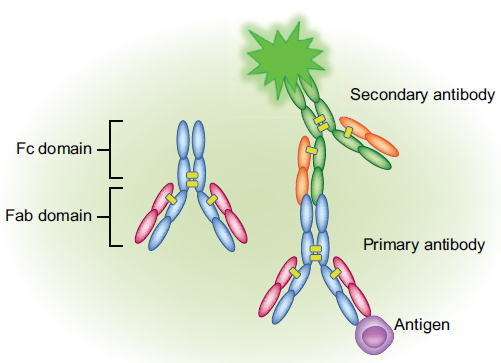
\includegraphics[scale=0.5]{Figures/Domain/antibodies}
	\rule{35em}{0.5pt}
	\caption[Illustration of antibody structure]{Illustration of antibody structure (from \cite{OdellCook2013})}
	\label{fig:AntibodyIllustration}

\end{figure}

The immune system can sometimes suffer from different disorders. A disorder of special importance to this Thesis is  \textit{autoimmunity}. Autoimmunity results in the disability of the immune system to recognize an organism's healthy tissue, and therefore attacks normal tissues as if they were foreign organisms. In the case of autoimmunity, antibodies are called antinuclear antibodies. We can observe those antibodies by using indirect immunofluorescence. \\

\subsection{Indirect Immunofluorescence}

As it was already mentioned, the indirect detection is the main focus of the thesis. Indirect immunofluorescence is a diagnostic methodology based on image analysis that reveals the presence of autoimmune diseases by searching for antibodies in the patient serum. Indirect immunofluorescence is a two-step technique, in which a primary, unlabeled antibody binds to the target, after which a fluorophore-labeled\footnote{fluorophore-labeling is a method to color the antibodies so they can be observed under the microscope} second antibody is used to detect the first antibody (figure \ref{fig:AntibodyIllustration}, right). Indirect immunofluorscence is more sensitive than a direct one because more than one secondary antibody can bind to each primary antibody, which amplifies the fluorescence signal. \\

As a result of its effectiveness,there has been a growing demand for diagnostic tests for systemic autoimmune diseases. Unfortunately,  IIF still remains a subjective method that depends too heavily on the experience and expertise of the physician. The main reasons causing the problems are:
\begin{itemize}
	\item the lack of quantitative information supplied to physicians
	\item varieties of reading systems and optics
	\item the photo-bleaching effect caused by a light source irradiating the cells over a short period of time
	\item the low reproducibility of the diagnostic protocol.
\end{itemize}

\subsection{Putting it all together}

The focus of this thesis is on the Antinuclear antibodies  test (ANA), which plays the main role in the serological\footnote{Further explanation} diagnosis of autoimmune disease. ANAs are directed against a variety of antigens and can be detected in patient serum through laboratory tests. IIF uses the human epithelial (HEp-2) substrate, which bonds with serum antibodies forming a molecular complex. This complex then reacts with human immunoglobulin \footnote{Immunoglobulin is a specific type of antibody created by plasma cells} and becomes visible under a fluorescence microscope which reveals the antigen-antibody reaction. \\

The procedure of ANA starts with  fluorescence intensity classification, a segmentation step is not a part of ANA procedure. The Center for Disease Control and Prevention in Atlanta,USA have published  guidelines \cite{nakamura1996quality} for scoring the intensity. The score ranges from 0 to 4+ as follows:
\begin{itemize}
	\item 4+ : brilliant green (maximal fluorescence)
	\item 3+ : less brilliant green fluorescence
	\item 2+ : defined pattern but diminished fluorescence
	\item 1+ : very subdued fluorescence
	\item 0 : negative.
\end{itemize}

Although the guidelines provide  very detailed instructions, in \cite{Rigon2007} Rigon et al. analyzed the variability between a set of physician's fluorescence intensity  classifications. Their work has shown a big variance of classifications made by physicians on the same dataset, so they suggested to classify the fluorescence intensity into three classes, namely negative, intermediate and positive. This work follows the protocol. \\

The final step consists of staining pattern recognition. As shown in figure \ref{fig:CellExamples}, there are several patterns that may be observed. \cite{FoggiaBenchmarks2013} and \cite{Perner02miningknowledge} provide a description of all staining patterns which is a valuable input taking into consideration a human interpretable perspective of this step. A summary is presented here:
\begin{itemize}

	\item \textbf{Centromere}: characterized by several discrete speckles ( $\sim$ 40 - 60) distributed throughout the interphase\footnote{The interphase is the nonmitotic phase of the cell cycle in which the cell spends the majority of its time and performs the majority of its purposes} nuclei and characteristically found in the condensed nuclear chromatin during mitosis as a bar of closely associated speckles.
	
	\item \textbf{Nucleolar}: characterized by clustered large granules in
the nucleoli of interphase cells which tend towards homogeneity, with less than six granules per cell.

	\item \textbf{Homogeneous}: characterized by a diffuse staining of the interphase nuclei and staining of the chromatin of mitotic cells.
	
	\item \textbf{Fine Speckled}: characterized by a fine granular nuclear staining of the interphase cell nuclei.
	
	\item \textbf{Coarse Speckled}: characterized by a coarse granular nuclear staining of the interphase cell nuclei.
	
	\item \textbf{Cytoplasmatic}: characterized by a highly irregular shape and large granule in the nucleoli

\end{itemize}


%------------------------------------------%
%                                          %
%           MACHINE LEARNING               %
%                                          %
%------------------------------------------%

\section{Machine learning}